\documentclass[11pt,letterpaper]{article}
\usepackage[lmargin=1in,rmargin=1in,tmargin=1in,bmargin=1in]{geometry}
\usepackage{../style/homework}
\usepackage{../style/commands}
\setbool{quotetype}{true} % True: Side; False: Under
\setbool{hideans}{false} % Student: True; Instructor: False

% -------------------
% Content
% -------------------
\begin{document}

\homework{1: Due 02/13 (14)}{In learning you will teach, and in teaching you will learn.}{Phil Collins}

% Problem 1
\problem{10} Let $\mathcal{U}= \{ -10, -9, \ldots, 9, 10 \}$. Define the following subsets of $\mathcal{U}$:
	\[
	\begin{aligned}
	A&= \{ -2, 0, 5, 10 \} \\
	B&= \text{even numbers in } \mathcal{U} \\
	C&= \{ -9, -7, -5, -3, -1, 1, 3, 5, 7, 9 \} \\
	D&= \text{positive prime numbers in } \mathcal{U} \\
	E&= \{ -5, -4, \ldots, 4, 5 \} 
	\end{aligned}
	\]
Using the sets defined above, answer the following: 
        \begin{enumerate}[(a)]
        \item $A \cap B$
        \item $B \cup E$
        \item $E - A$
        \item $B^c$
        \item $|D|$
        \end{enumerate} \pspace

\sol 
\begin{enumerate}[(a)]
\item The set $A \cap B$ is the collection of objects that are elements of \textit{both} $A$ and $B$. But then we have\dots
	\[
	A \cap B= \{ -2, 0, 10 \}
	\] \pspace

\item The set $B \cup E$ is the collection of objects that are elements of either $B$ or $E$. But then we have\dots
	\[
	B \cup E= \{ -10, -8, -6, -5, -4, -3, -2, -1, 0, 1, 2, 3, 4, 5, 6, 8, 10 \}
	\] \pspace

\item The set $E - A$ is the collection of objects that are elements of $E$ but \textit{not} elements of $A$. But then we have\dots
	\[
	E - A= \{ -5, -4, -3, -1, 1, 2, 3, 4 \}
	\] \pspace

\item The set $B^c$ is the collection of objects that are elements (of $\mathcal{U}$) that are \textit{not} elements of $B$. But then we have\dots
	\[
	B^c= \{ -9, -7, -5, -3, -1, 1, 3, 5, 7, 9 \}
	\] \pspace

\item The number $|D|$ is the cardinality or `size' of $D$; that is, $|D|$ is the number of distinct (unique) elements of $D$. But then as $D= \{ 2, 3, 5, 7 \}$, we have $|D|= 4$. 
\end{enumerate}



\newpage



% Problem 2
\problem{10} Define the following sets:
	\[
	\begin{aligned}
	A&= \text{set of multiples of 3} \\
	B&= \text{set of divisors of 30} \\
	C&= \text{set of even numbers less than 10} 
	\end{aligned}
	\]
Using the sets defined above, answer the following:
        \begin{enumerate}[(a)]
        \item List the elements of $B$.
        \item Give the largest element of $A$ less than 50 and the largest negative element of $A$.
        \item What are the elements of $B - A$?
        \item What are the elements of $A \cap B$?
        \item Are $B$ and $C$ disjoint? Explain. 
        \end{enumerate} \pspace

\sol 
\begin{enumerate}[(a)]
\item The divisors of 30 are 1, 2, 3, 5, 6, 10, 15, and 30. Therefore, 
	\[
	B= \{ 1, 2, 3, 5, 6, 10, 15, 30 \}
	\] \pspace

\item The largest element of $A$ less than 50 will be the largest multiple of 3 that is less than 50. We know that 50 is not divisible by 3, nor is 49. However, as $48= 16(3)$, we know that 48 is divisible by 3. Therefore, 48 is the largest element of $A$ (an integer divisible by 3) that is less than 50. The negative elements of $A$, i.e. the negative integers that are a multiple of 3, are $-3, -6, -9, -12, -15, \ldots$. The largest of these negative multiples of 3 is $-3$. \pspace

\item The objects of $B - A$ are the elements of $B$ that are \textit{not} elements of $A$. The elements of $B$ are the divisors of 30 and the elements of $A$ are the multiples of 3. Then the elements of $B - A$ are the integers that are divisors of 30 that are not multiples of 3. But then we have\dots
	\[
	B - A= \{ 1, 2, 5, 10 \}
	\]


\item The objects of $A \cap B$ are objects that are elements of \textit{both} $A$ and $B$. The elements of $A$ are the multiples of 3 and the elements of $B$ are the divisors of 30. Therefore, the elements of $A \cap B$ are the integers that are multiples of 3 that are also divisors of 30. But then we have\dots
	\[
	A \cap B=  \{ 3, 6, 15, 30 \}
	\] \pspace

\item The sets $B$ and $C$ are disjoint if $B \cap C= \emptyset$; that is, if there is no integer that is an element of both $B$ and $C$. However, 2 is an even number less than 10 so that $2 \in C$. But 2 is also a divisor of 30 so that $2 \in B$. This shows $2 \in B \cap C$ so that $B \cap C \neq \emptyset$. Therefore, $B$ and $C$ are not disjoint. 
\end{enumerate}



\newpage



% Problem 3
\problem{10} Look at the Venn diagram given below:
	\[
	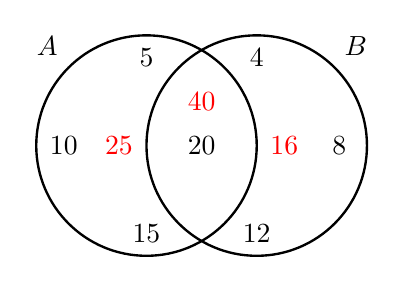
\begin{tikzpicture}[scale=0.7]
	\draw[line width=0.03cm] (-1,0) circle (2);
	\draw[line width=0.03cm] (1,0) circle (2);
	\node at (-2.8,1.8) {$A$}; 
	\node at (-1,1.6) {$5$}; \node at (-2.5,0) {$10$}; \node at (-1,-1.6) {$15$};
	\node at (2.8,1.8) {$B$};
	\node at (1,1.6) {$4$}; \node at (2.5,0) {$8$}; \node at (1,-1.6) {$12$};
	\node at (0,0) {$20$};
	
	\node at (-1.5,0) {\color{red}\bfseries$25$};
	\node at (1.5,0) {\color{red}\bfseries$16$};
	\node at (0,0.8) {\color{red}\bfseries$40$};
	\end{tikzpicture}
	\]
Use this diagram to answer the following:
	\begin{enumerate}[(a)]
	\item Assuming only a few of the elements of $A$ and $B$ are given in the diagram above, describe what the sets $A$ and $B$ likely represent.
	\item Place the numbers $25$, $16$, and $40$ in appropriate places in the given Venn diagram. 
	\item Using words, explain what numbers go in the same region of the Venn diagram in which $20$ is found.
	\item Using words, explain what numbers go in the same region of the Venn diagram in which $4$, $8$, and $12$ are found.
	\item What numbers would be placed outside of both the regions $A$ and $B$? Give an example.  
	\end{enumerate} \pspace

\sol 
\begin{enumerate}[(a)]
\item The elements of $A$ are the integers 5, 10, 15, and 20. We may then possibly describe $A$ as the set of positive multiples of 5. The elements of $B$ are the integers 4, 8, 12, 20. We may then possibly describe $B$ as the set of positive multiples of 4. \pspace

\item Because 25 is a multiple of 5 but not 4, 25 belongs only in the set $A$. Because 16 is a multiple of 4 but not a multiple of 5, 16 belongs only in the set $B$. Because 40 is a multiple of both 5 and 4, 40 belongs in both the set $A$ and $B$. We then place 25, 16, and 40 in appropriate places in the diagram above. 

\item The number 20 is in the overlap of the sets $A$ and $B$. But then this region represents the collection of elements that are in $A$ and $B$, i.e. $A \cap B$. This is the collection of integers that are both in $A$ (hence a positive multiple of 5) and in $B$ (hence a positive multiple of 4). To be a multiple of 4 and 5 implies that you are a multiple of $\text{lcm}(4, 5)= 20$. Then the region with 20 is the set of positive integers that are a multiple of 20. \pspace

\item The numbers 4, 8, 12 are in $B$, i.e. are a positive multiple of 4, but are not in $A$, i.e. they are not a positive multiple of 5. But then region containing 4, 8, and 12 are the positive integers which are a multiple of 4 but not a multiple of 5, i.e. an element of the set $B - A$. \pspace

\item The region outside the circles $A$ and $B$ consist of the elements that are not in $A$, i.e. not a positive multiple of 5, and not in $B$, i.e. not a positive multiple of 4. But then this region consists of the positive integers which are not multiples of 4 and not multiples of 5. For example, 1, 2, 3, 6, 7, 9, 11, etc. are all elements of the region outside the circles $A$ and $B$. 
\end{enumerate}



\newpage



% Problem 4
\problem{10} You are working with a student named Lucy. You give her the following sets: $A= \{ a, b, c, d, a \}$ and $B= \{ c, d, e, f \}$. 
	\begin{enumerate}[(a)]
	\item Lucy states that the cardinality of $A$ is 5. Explain why Lucy is wrong. How might you correct her?
	\item You ask Lucy to find $A \cup B$ and she states that this is $\{ c, d \}$. What has Lucy done wrong?
	\item Cameron overhears Lucy's answer in (b) and shouts that the answer is $\{ a, b, e, f \}$. How has Cameron misunderstood the mathematical word \textit{or} in this context? 
	\item Both Lucy and Cameron state that you cannot find $A - B$ because they are filled with letters and you cannot subtract letters. Explain what they have misunderstood about sets. 
	\end{enumerate} \pspace

\sol 
\begin{enumerate}[(a)]
\item The cardinality, or size, of a set is the number of distinct (unique) elements of a set. Repetition or order of elements of a set do not matter. But then we know that $A= \{ a, b, c, d, a \}= \{ a, a, b, c, d \}= \{ a, b, c, d \}$. But then $A$ only has 4 distinct elements so that $|A|= 4$. Lucy is misunderstanding that it is not the number of `objects' of $A$ that matters; it is the number of \textit{distinct} objects of $A$. You should explain to her that she should eliminate duplicates before counting the elements of a set. \pspace

\item The set $A \cup B$ should consist of the elements that are in either $A$ or $B$. The set $A \cap B$ is the set of elements that are in both $A$ and $B$. Notice that $c$ is in $A$ and $B$ and $d$ is in $A$ and $B$. There are no other elements that are in both $A$ and $B$. But then $A \cap B= \{ c, d \}$. It is then likely that Lucy has confused the symbols $\cup$ and $\cap$. \pspace

\item The set $A \cup B$ should consist of the elements that are in $A$ or $B$. However, `or' in Mathematics always refers to one or the other or both; that is, the elements of $A \cup B$ are the elements in either $A$ or $B$. The elements `a' and `b' are only in $A$ and the elements `e' and `f' are only in $B$. Cameron then seems to be treating the word `or' as `exclusive-or' and is not using it in the mathematical sense. \pspace

\item They are treating `$-$' as if it refers to subtraction. However, in this context, we should treat `$-$' as `removing.' The set $A - B$ is then the collection of elements of $A$ after having `removed' the elements that are in $B$; that is, the set $A - B$ is the collection of elements of $A$ that are not elements of $B$. 
\end{enumerate}


\end{document}